%==============================================
\subsection{Ranking of Potential Blocking Gaps}\label{subsec:gap}

When the condition in~\eqref{eq:wccg_criterion} fails, the vehicle cannot
reach~$\mathbf{s}_\texttt{V}^{\texttt{G}}$ from
$\mathbf{s}_\texttt{V}^{\texttt{S}}$ through a $W$--clear path
$\mathcal{P}^W_\texttt{V}$. In this case, the planner must prioritize
\emph{blocking gaps} on the reachable frontier of $\mathcal{G}_W$. The goal of
this module is to provide an ordered list of such gaps, ranked by their
predicted cost to eventually yield a feasible path, which serves
as a critical guidance for the hybrid search in the sequel.

\subsubsection{Frontier Extraction and Candidate Gaps}
A BugPlanner query on $\mathcal{G}_W$, given
$(\mathbf{s}_\texttt{V}^{\texttt{S}},\mathbf{s}_\texttt{V}^{\texttt{G}},W)$,
either confirms connectivity or returns a counter--clockwise frontier loop
$\mathcal{L}$ that separates the two endpoints. The bridge--bridge edges
visible on $\mathcal{L}$ form the first--hop candidate set
$\mathcal{G}(\mathcal{L})\triangleq\{g_1,\cdots,g_K\}$,
where each $g_k$ is a reachable candidate gap. These candidates are the inputs
to the ranking module, while the output will be an ordered list of the same
set sorted by predicted cost.

\subsubsection{Evaluation for Immediate Cost}
Each candidate $g\in\mathcal{G}(\mathcal{L})$ is evaluated by combining the
cost for the robots to reach the gap and the effort required to widen it.
Let $\mathbf{s}_{\mathcal{R}}$ be the current robot positions,
and $\mathbf{o}_g$ as the outside insertion point of gap $g$. The
resulting one--hop cost is given by:
\begin{equation}\label{eq:step_cost}
\mathsf{C}\big(g \mid \mathcal{L}, \mathbf{s}_{\mathcal{R}}\big)
=\lambda_\texttt{t}\,\mathsf{C}_\texttt{t}\!\left(\mathbf{s}_{\mathcal{R}},\mathbf{o}_g\right)
+\lambda_\texttt{p}\,\mathsf{C}_\texttt{p}(g),
\end{equation}
where $\lambda_\texttt{t},\lambda_\texttt{p}>0$ are weighting factors
for the transition and pushing costs, respectively;
function $\mathsf{C}_\texttt{t}(\cdot)$ denotes the collision-free
distance between two points;
and the function~$\mathsf{C}_\texttt{p}(\cdot)$ measures the widening effort,
which increases when the gap is narrower than $W$,
or when the adjacent obstacles are heavier as scaled by a mass factor
based on the adjacent movable
obstacles~$\Omega_u,\Omega_v\in \boldsymbol{\Omega}$ with masses $\mathsf{M}_u$ and $\mathsf{M}_v$.

%------------------------------
\begin{figure}[t!]
  \centering
  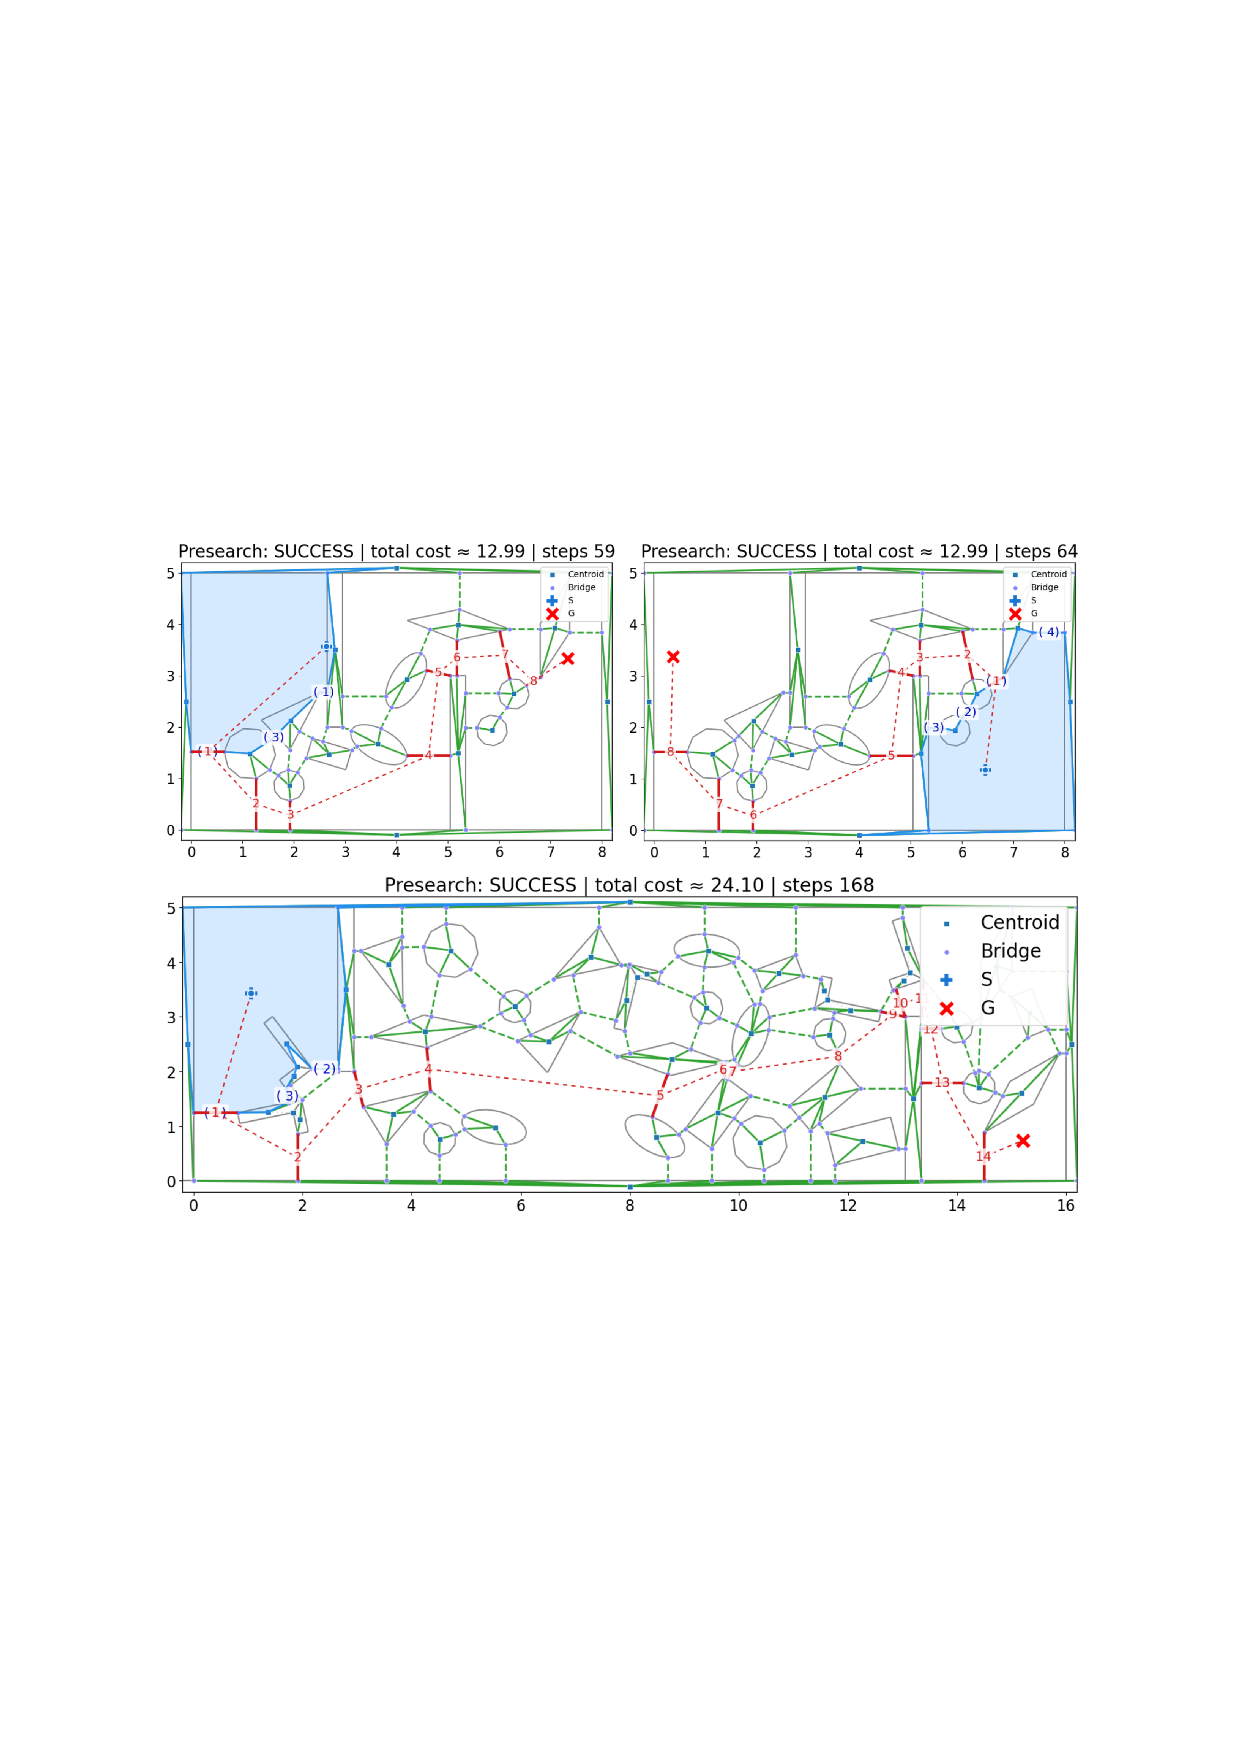
\includegraphics[width=\linewidth]{figures/presearch.pdf}% or {presearch.pdf}
  \vspace{-0.15in}
  \caption{
  Illustration for {the ranking of potential gaps.}
  Each panel overlays the WCCG together with the currently selected face (light blue).
  The algorithm (i) extracts the frontier loop from BugPlanner,
  (ii) enumerates candidate bridge--bridge gaps on the loop,
  (iii) assigns local first-hop ranks (blue numbers),
  and (iv) simulates a short presearch to predict the full gap-crossing sequence (red numbers).
  \textbf{Top:} identical environment with start and goal swapped;
  the resulting gap sequences are symmetric with identical predicted cost at $12.99$;
  \textbf{Bottom:} a larger map with about $30$ obstacles, where presearch returns a 14-gap sequence
  of predicted cost at $24.10$.
}

  \label{fig:presearch}
  \vspace{-0.1in}
\end{figure}
%------------------------------

\subsubsection{Long-term Cost w.r.t. Goal}
Furthermore, to prioritize gaps closer to the goal, a heuristic is added to the evaluation,
i.e.,
$h(g)=\eta\,\big\|\mathbf{o}(g)-\mathbf{s}_\texttt{V}^{\texttt{G}}\big\|$,
where $\eta>0$ is a scaling constant. Lastly, a short A$^\star$-style presearch virtually crosses
each candidate gap, recomputes the next frontier, and continues for a limited
beam width and depth. The predicted cost-to-connect is given by:
\begin{equation}\label{eq:pred_cost}
\widehat{\mathsf{Cost}}(g)\triangleq
\mathsf{C}\!\big(g \mid \mathcal{L},\mathbf{s}_{\mathcal{R}}\big)
+\!\!\!\sum_{g'\in\Pi^\star(g)}\!\!\!\big{\{}\mathsf{C}(g' \mid \cdot)+h(g')\big{\}},
\end{equation}
where $\Pi^\star(g)$ is the sequence of subsequent gaps discovered after
virtually crossing $g$;
the dots indicate updated inputs along that rollout;
and the scalar score $\widehat{\mathsf{Cost}}(g)>0$ for each candidate gap.
Consequently,
the final output of this module is the ranked list of candidate gaps, i.e.,
$\textsf{Rank}\big(\mathcal{G}(\mathcal{L})\big)
\triangleq \textbf{argsort}_{g\in\mathcal{G}(\mathcal{L})}\widehat{\mathsf{Cost}}(g)$,
which sorts $\mathcal{G}(\mathcal{L})$ in ascending predicted cost. This
ordered set is passed to the hybrid search module, such that only the
promising gaps are expanded first.

\begin{remark}[Practical Heuristics]\label{remark:gap}
Efficiency of the above ranking procedure can be improved by
caching frontier loops, storing the transitions
$(\mathcal{L},g)\mapsto\mathcal{L}'$, and accelerating the edge queries with
axis-aligned bounding-box culling. With a small beam width and depth
(typically around $8$), the runtime of ranking remains negligible compared to
the cost of simulation-based validation. \hfill$\blacksquare$
\end{remark}




%% %------------------------------
%% \begin{algorithm}[t]
%% \small
%% \caption{Frontier Presearch for Gap Ranking (compact)}
%% \label{alg:gap-ranking}
%% \DontPrintSemicolon
%% \SetKwInOut{Input}{In}\SetKwInOut{Output}{Out}
%% \Input{$\mathbf{s}^{\texttt{S}}$, $\mathbf{s}^{\texttt{G}}$, WCCG, $\lambda_{\mathrm{trans}}$, $\lambda_{\mathrm{push}}$}
%% \Output{First-hop gaps ranked by predicted cost}
%% $(\mathcal{L},\texttt{conn})\!\leftarrow\!\texttt{BugFrontier}(\mathbf{s}^{\texttt{S}},\mathbf{s}^{\texttt{G}})$;\;
%% \If{\texttt{conn}}{\Return $\emptyset$}
%% $\mathcal{C}\!\leftarrow$ bridge–bridge gaps on $\mathcal{L}$;\;
%% \For{$g\in\mathcal{C}$}{
%%   $J_1\!\leftarrow\!\lambda_{\mathrm{trans}}\mathsf{C}_{\mathrm{trans}}+\lambda_{\mathrm{push}}\kappa(g)[\max(0,W-w(g))+\delta]$;\;
%%   $(\texttt{succ},J_{\mathrm{tail}})\!\leftarrow\!\texttt{PresearchAfter}(g)$;\;
%%   $\widehat{\mathrm{Cost}}(g)\!\leftarrow\!J_1+\big(\texttt{succ}?J_{\mathrm{tail}}:\infty\big)$;\;
%% }
%% \Return $\mathrm{argsort}_{g\in\mathcal{C}}\widehat{\mathrm{Cost}}(g)$ (asc.)\;
%% \end{algorithm}
